\documentclass[12pt]{article}

\usepackage{amsmath,amsthm,amsfonts,amssymb,amsxtra}
\usepackage{pgf,tikz}
\usetikzlibrary{arrows}
\renewcommand{\theenumi}{(\alph{enumi})} 
\renewcommand{\labelenumi}{\theenumi}

\pagestyle{empty}
\setlength{\textwidth}{7in}
\setlength{\oddsidemargin}{-0.5in}
\setlength{\topmargin}{-1.0in}
\setlength{\textheight}{9.5in}

\newtheorem{problem}{Problem}

\begin{document}

\noindent{\large\bf MATH 141}\hfill{\large\bf Exam\#1.}\hfill{\large\bf
  Fall 2008}\hfill{\large\bf Page 1/7}\hrule

\bigskip
\begin{center}
  \begin{tabular}{|ll|}
    \hline & \cr
    {\bf Name: } & \makebox[12cm]{\hrulefill}\cr & \cr
    {\bf 4-digit code:} & \makebox[12cm]{\hrulefill}\cr & \cr
    \hline
  \end{tabular}
\end{center}
\begin{itemize}
\item Write your name and the last 4 digits of your SSN in the space provided above.
\item The test has seven (7) pages, including this one.
\item Enter your answer in the box(es) provided.
\item You must show sufficient work to justify all answers unless
  otherwise stated in the problem.  Correct answers with inconsistent
  work may not be given credit.
\item Credit for each problem is given in parentheses at the right of
  the problem number.
\item No books, notes or calculators may be used on this test.
\end{itemize}
\hrule

\begin{center}
  \begin{tabular}{|c|c|c|}
    \hline
    &&\cr
    {\large\bf Page} & {\large\bf Max.~points} & {\large\bf Your points} \cr
    &&\cr
    \hline
    &&\cr
    {\Large 2} & \Large 20 & \cr
    &&\cr
    \hline
    &&\cr
    {\Large 3} & \Large 15 & \cr
    &&\cr
    \hline
    &&\cr
    {\Large 4} & \Large 15 & \cr
    &&\cr
    \hline
    &&\cr
    {\Large 5} & \Large 30 & \cr
    &&\cr
    \hline
    &&\cr
    {\Large 6} & \Large 10 & \cr
    &&\cr
    \hline
    &&\cr
    {\Large 7} & \Large 10 & \cr
    &&\cr
    \hline\hline
    &&\cr
    {\large\bf Total} & \Large 100 & \cr
    &&\cr
    \hline
  \end{tabular}
\end{center}
\newpage

%%%%%%%%%%%%%%%%%%%%%%%%%%%%%%%%%%%%% Page 1
\noindent{\large\bf MATH 141}\hfill{\large\bf Exam\#1.}\hfill{\large\bf
  Fall 2008}\hfill{\large\bf Page 2/7}\hrule

\bigskip
{\problem[5 pts] \em Find $f(3)$ and $f(\pi)$ for}
$f(x) = 
\begin{cases}
 \sqrt{x+1} & \text{if } x\geq 1,\\
3 & \text{if } x<1.
\end{cases}$
\vspace{1cm}
\begin{flushright}
  \begin{tikzpicture}
    \draw (-1cm,0.5cm) node {$f(\pi) =$};
    \draw (0cm,0cm) rectangle (5cm,1.2cm);
    \draw (-1cm,2cm) node {$f(3) =$};
    \draw (0cm,1.4cm) rectangle (5cm,2.6cm);
  \end{tikzpicture}
\end{flushright}
\hrule
{\problem[5 pts] \em Find the domain of $f(x) = 2 + \sqrt{x-1}$.}
\vspace{4cm}
\begin{flushright}
  \begin{tikzpicture}
    \draw (-1cm,0.5cm) node {domain $=$};
    \draw (0cm,0cm) rectangle (5cm,1.2cm);
  \end{tikzpicture}
\end{flushright}
\hrule
{\problem[10 pts] \em Express the function $f(x) = \lvert x \rvert + 3x
  + 1$ in piecewise form without using absolute values.}
\vspace{8cm}
\begin{flushright}
  \begin{tikzpicture}
    \draw (-1cm,0.5cm) node {$f(x) = {\Biggr\{}$};
    \draw (0cm,-0.6cm) rectangle (5cm,1.8cm);
  \end{tikzpicture}
\end{flushright}
\newpage

%%%%%%%%%%%%%%%%%%%%%%%%%%%%%%%%%%%%% Page 2
\noindent{\large\bf MATH 141}\hfill{\large\bf Exam\#1.}\hfill{\large\bf
  Fall 2008}\hfill{\large\bf Page 3/7}\hrule

\bigskip
{\problem[5 pts] \em Let $f(x) = x^2 + 3$ and $g(x) = \sqrt{x}$. Find
  $\big( g \circ f\big)(x)$.}
\vspace{2cm}
\begin{flushright}
  \begin{tikzpicture}
    \draw (-1.25cm,0.5cm) node {$ \big(g \circ f\big)(x) =$};
    \draw (0cm,0cm) rectangle (5cm,1.2cm);
  \end{tikzpicture}
\end{flushright}
\hrule
{\problem[5 pts] \em Classify the function $f(x) = x^5$ as even, odd
  or neither.} 
\vspace{3cm}
\begin{flushright}
  \begin{tikzpicture}
    \draw (-0.75cm,0.5cm) node {$f$ is};
    \draw (0cm,0cm) rectangle (5cm,1.2cm);
  \end{tikzpicture}
\end{flushright}
\hrule
{\problem[5 pts] \em Find the amplitude and period of}
\begin{equation*}
y = 3 \cos \big( 2x + \tfrac{\pi}{2} \big).
\end{equation*}
\vspace{6cm}
\begin{flushright}
  \begin{tikzpicture}
    \draw (-1.25cm,0.5cm) node {$\text{amplitude} =$};
    \draw (0cm,0cm) rectangle (5cm,1.2cm);
    \draw (-1cm,2cm) node {$\text{period} =$};
    \draw (0cm,1.4cm) rectangle (5cm,2.6cm);
  \end{tikzpicture}
\end{flushright}
\newpage

%%%%%%%%%%%%%%%%%%%%%%%%%%%%%%%%%%%%% Page 3
\noindent{\large\bf MATH 141}\hfill{\large\bf Exam\#1.}\hfill{\large\bf
  Fall 2008}\hfill{\large\bf Page 4/7}\hrule

\bigskip
{\problem[5 pts] \em Solve for $x$: $\log (3x) - 3 \log (x^{-1/3}) =
  \log 27$.}
\vspace{3cm}
\begin{flushright}
  \begin{tikzpicture}
    \draw (-0.75cm,0.5cm) node {$x =$};
    \draw (0cm,0cm) rectangle (5cm,1.2cm);
  \end{tikzpicture}
\end{flushright}
\hrule
{\problem[10 pts] Sketch the curve by eliminating the parameter
  (i.e.~try to write $y=f(x)$), and indicate the direction of
  increasing $t$} 
\begin{equation*}
x=\sqrt{t},\quad y=\tfrac{3}{4}t+3\quad (0 \leq t \leq 4).
\end{equation*}
\begin{center}
\begin{tikzpicture}
\clip (0cm, 0cm) rectangle (10cm,10cm);
\begin{scope}[xshift=5cm, yshift=5cm]
\draw[gray, very thin, step=0.5cm] (-4.4cm,-4.4cm) grid (4.4cm, 4.4cm);
\draw[<->, very thick] (0cm, -5cm) -- (0cm, 5cm);
\draw[<->, very thick] (-5cm, 0cm) -- (5cm, 0cm);
\end{scope}
\end{tikzpicture}
\end{center}
\newpage

%%%%%%%%%%%%%%%%%%%%%%%%%%%%%%%%%%%%% Page 4
\noindent{\large\bf MATH 141}\hfill{\large\bf Exam\#1.}\hfill{\large\bf
  Fall 2008}\hfill{\large\bf Page 5/7}\hrule

\bigskip
{\problem[30 pts] \em Compute the following limits:}
\vspace{1cm}

\noindent
\begin{tikzpicture}
\draw (4cm,14cm) node{
(a) $\displaystyle{\lim_{x \to 1} \frac{x^2-2x-8}{x^2-4}} = \mbox{}$ };
\draw (6cm,13.4cm) rectangle (11cm,14.6cm);
\draw (4cm, 10cm) node{
(b) $\displaystyle{\lim_{x \to \infty} \frac{x^2-2x-8}{x^2-4}} =
\mbox{}$}; 
\draw (6.1cm, 9.4cm) rectangle (11.1cm, 10.6cm); 
\draw (4cm, 3cm) node{
(c) $\displaystyle{\lim_{x \to \infty} \Big( 1 + \frac{5}{x} \Big)^{3x}} = \mbox{}$}; 
\draw (6cm, 2.4cm) rectangle (11cm, 3.6cm);
\end{tikzpicture}
\newpage


%%%%%%%%%%%%%%%%%%%%%%%%%%%%%%%%%%%%% Page 5
\noindent{\large\bf MATH 141}\hfill{\large\bf Exam\#1.}\hfill{\large\bf
  Fall 2008}\hfill{\large\bf Page 6/7}\hrule

\bigskip
{\problem[10 pts] \em Recall the ``$\varepsilon$--$\delta$'' definition of limit:
\begin{center}
\begin{tikzpicture}
\draw (0.5\linewidth, 0cm) node[text justified, text width=0.5\linewidth, draw, rounded corners] {
We write $\displaystyle{\lim_{x\to a}} f(x) = L$ if for all $\varepsilon
> 0$ there exists $\delta >0$ such that $\lvert x - a \rvert < \delta$
implies $\lvert f(x) - L \rvert < \varepsilon$.}; 
\end{tikzpicture}
\end{center}
Use this definition to prove that $\displaystyle{\lim_{x \to 4} 5x-2 =
  18}$.}
\newpage

%%%%%%%%%%%%%%%%%%%%%%%%%%%%%%%%%%%%% Page 6
\noindent{\large\bf MATH 141}\hfill{\large\bf Exam\#1.}\hfill{\large\bf
  Fall 2008}\hfill{\large\bf Page 7/7}\hrule

\bigskip
{\problem[10 pts] \em Find the value of the constant $k$ for which the following function is continuous everywhere:}
\begin{equation*}
f(x) = \begin{cases}
2k^2x^3 &\text{if }x<2, \\
x+32k-18 &\text{if }x \geq 2.
\end{cases}
\end{equation*}
\vspace{16cm}
\begin{flushright}
  \begin{tikzpicture}
    \draw (-1cm,0.5cm) node {$k =$};
    \draw (0cm,0cm) rectangle (5cm,1.2cm);
  \end{tikzpicture}
\end{flushright}

\end{document}
